% Chapter Template

\chapter{Ensayos y resultados} % Main chapter title
En este capítulo se detallan los ensayos realizados en las formaciones ferroviarias y en los talleres de Trenes Argentinos. El orden cronológico de los ensayos es distinto al del desarrollo del firmware. En este documento se ha presentado previamente el diseño de la solución para facilitar la comprensión del trabajo realizado. El desarrollo de la solución fue posterior a una serie de mediciones realizadas en los talleres que permitieron identificar parámetros clave del sistema. \\

En las secciones que siguen se explican las mediciones realizadas en las visitas a los talleres de Victoria y Castelar de Trenes Argentinos Operaciones. Luego se presenta un análisis de datos de las tramas relevadas y también las pruebas de integración propuestas para validar el desarrollo. \\


\label{Chapter4} % Change X to a consecutive number; for referencing this chapter elsewhere, use \ref{ChapterX}

%----------------------------------------------------------------------------------------
%	SECTION 1
%----------------------------------------------------------------------------------------

\section{Mediciones}

\section{Análisis de tramas}

\section{Pruebas en maqueta}

\subsubsection{Placa de control}

\begin{figure}[ht]
	\centering
	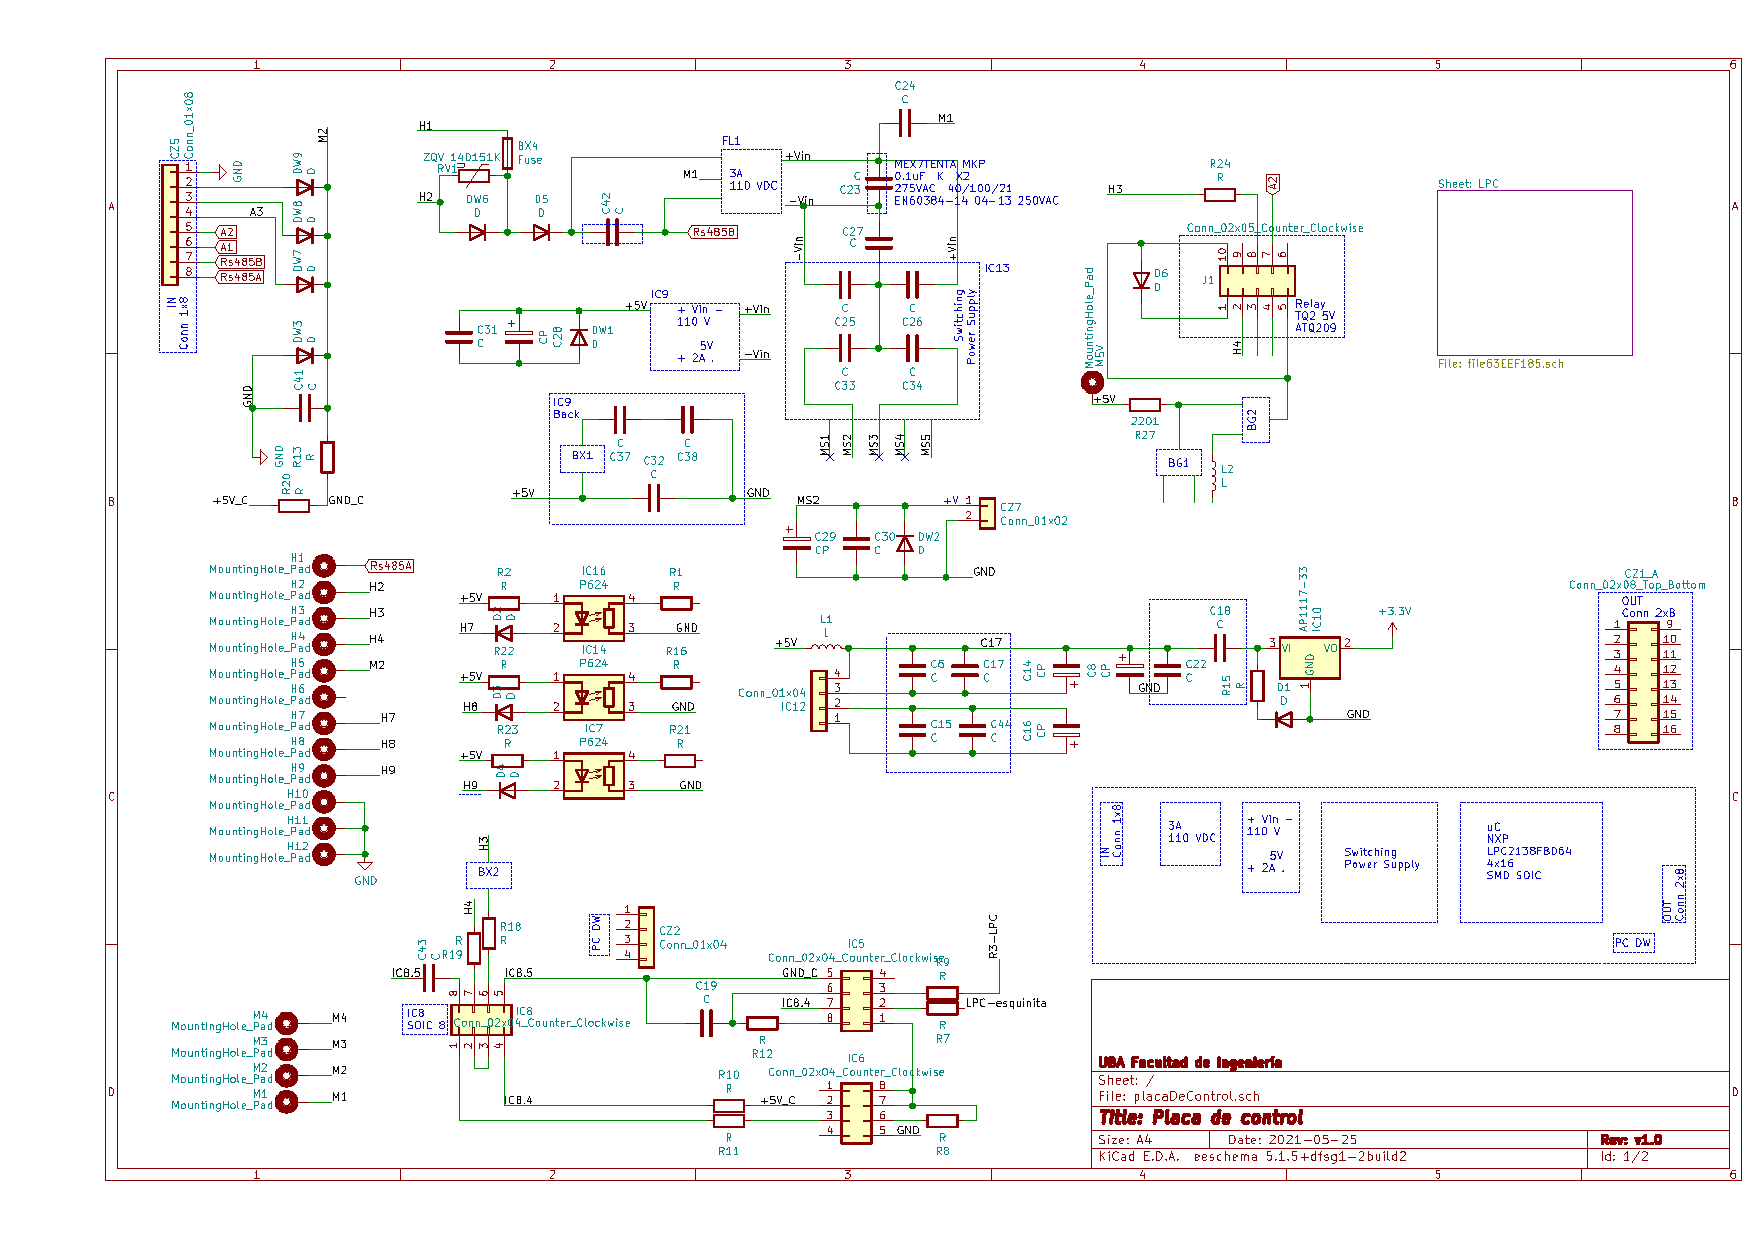
\includegraphics[width=1\textwidth]{./Figures/output.placaControl.pdf}
	\caption{Circuito esquemático de la placa de control de los carteles LED de salón.}
	\label{fig:schController}
\end{figure}


\begin{figure}[ht]
	\centering
	
\includegraphics[width=0.5\textwidth]{./Figures/diagramasTemporales.png}
	\caption{}
	\label{fig:diagramasTemporales}
\end{figure}

\section{Integración con red PIDS}

\section{Pruebas de campo}

\begin{figure}[ht]
	\centering
	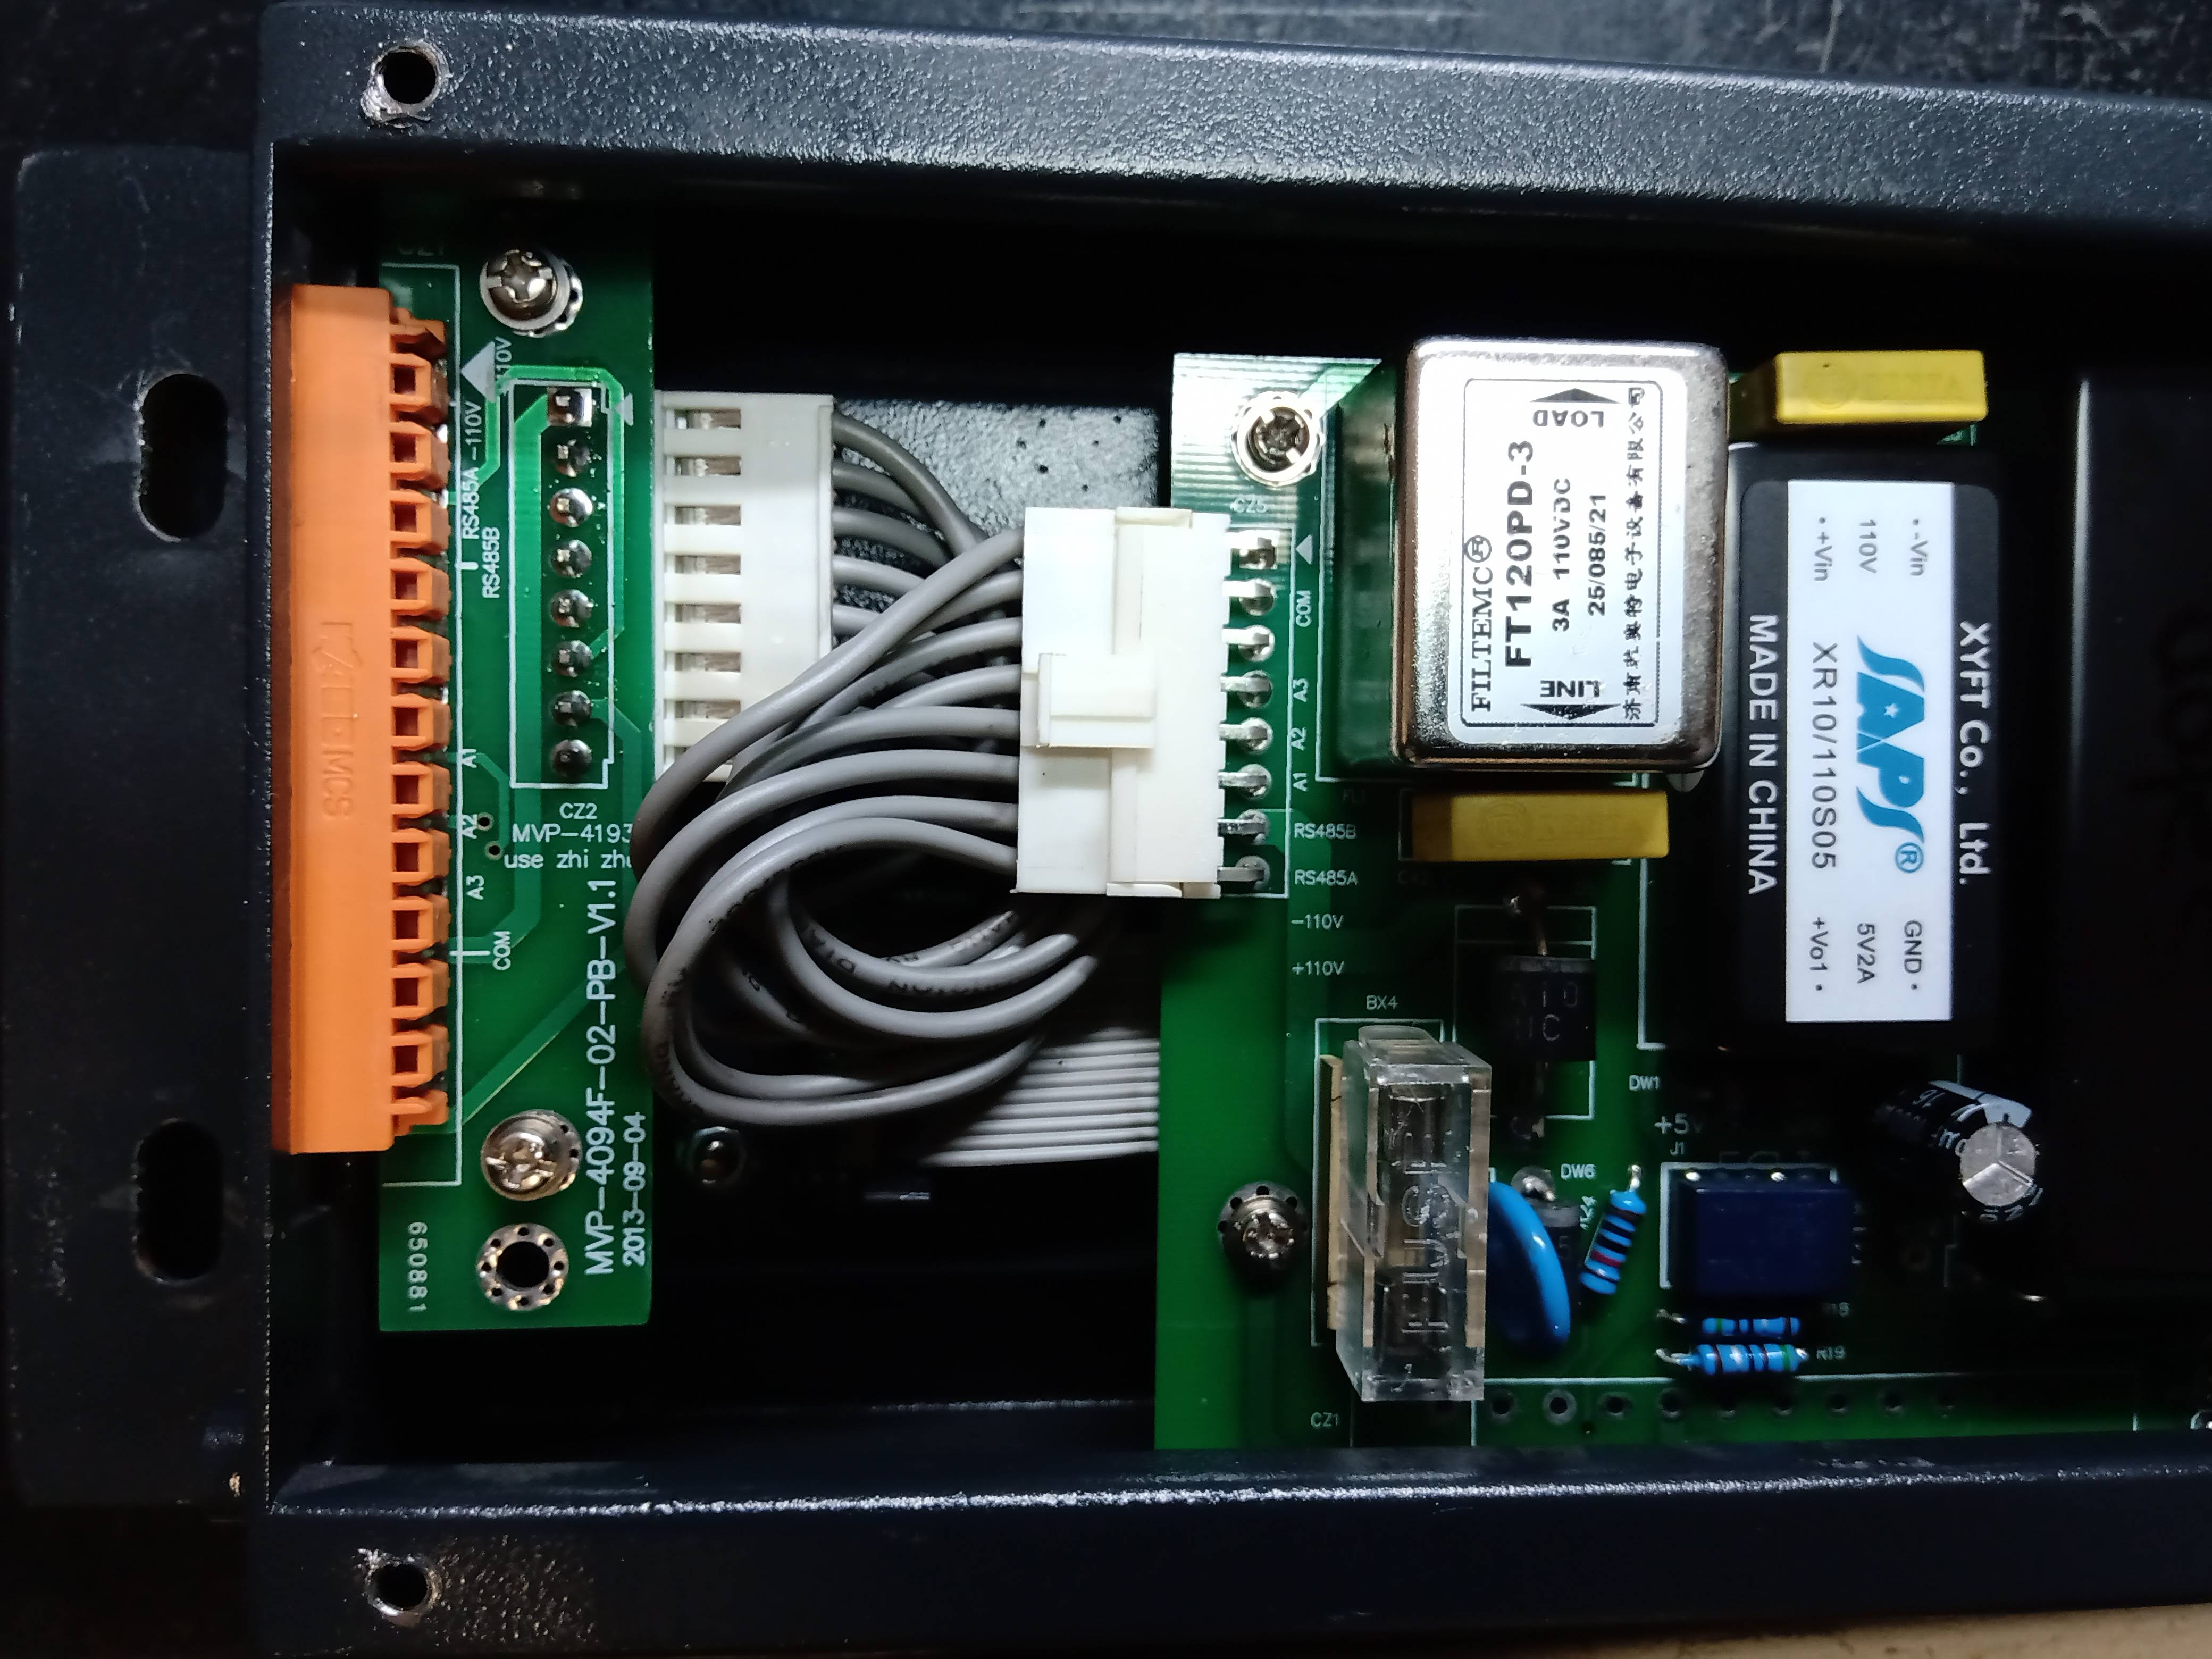
\includegraphics[width=1\textwidth]{./Figures/displayController.jpg}
	\caption{Fotografía del detalle de conexión de la placa de control de los carteles led de salón.}
	\label{fig:displayController}
\end{figure}